\chapter{Design}
The system is designed to handle a substantial volume of data with varying attributes in both number and type. 
There are several anime and manga entries that contains missing or incomplete information, and the system must be able to handle this,
avoiding meaningless memory occupation. To accommodate this, a Document Database was chosen for its flexibility and schema-less nature,
ease of use, and high-performance capabilities. This choice enables the execution of complex queries, 
including advanced filtering across different attribute types.
\\ \\
In addition, the implementation of social networking functionalities necessitated the use of a Graph Database. 
This allows for efficient traversal of relationships between entities and effectively manages connections between 
different entities such as users, anime, and manga.


\section{Document Database}

For the document database, we will use \textbf{MongoDB}. The decision to use a document database, 
specifically MongoDB,  was driven by its \textbf{flexibility} and \textbf{schema-less nature}, 
which allows for the storage of data with varying attributes in both number and type. 
This adaptability makes MongoDB ideal for handling diverse and dynamic data models.

\vspace{\baselineskip}

MongoDB also provides a \textbf{high-performance environment} for executing complex queries, 
reducing the need for joins and improving overall application performance by minimizing database 
access. This is particularly beneficial for applications like MangaVerse that require fast response 
times and can benefit from pre-computed relationships between entities. By storing embedded 
relationships directly within documents, MongoDB enables quicker data retrieval, enhancing user experience.

\vspace{\baselineskip}

To avoid normalized data, \textbf{data redundancy} is used to define relationships between entities.
Although this technique can lead to increased memory usage, it enables faster queries and fewer 
database accesses. For applications with high query complexity and rapidly growing data, 
such as MangaVerse, this is an optimal trade-off.

\vspace{\baselineskip}

To define \textbf{one-to-many relationships}, the documents linking pattern is used. 
In this pattern, one entity stores a list of the IDs of related entities, allowing for 
quick retrieval without multiple queries. This approach is used for retrieving reviews 
written by a user or reviews associated with a specific anime or manga. Additionally, document 
embedding is used for storing the latest reviews within the anime or manga documents, enabling 
fast access to this information when a user views the anime or manga page.

\vspace{\baselineskip}

The document database also includes other redundancies between collections and between the document
database and the graph database. For example, fields such as the number of likes for a manga or 
anime, the number of followers and followings for a user, and the average rating of media content
are stored redundantly. To maintain consistency without unnecessary database accesses, a flag 
called \textbf{'avg\_rating\_last\_update'} is used to indicate whether the average rating is 
up-to-date.

\vspace{\baselineskip}

MongoDB is also a \textbf{scalable database}, capable of handling large volumes of data and traffic. 
It supports distribution, providing \textbf{high availability}, \textbf{fault tolerance}, and \textbf{data integrity}. 
This means MongoDB can easily be scaled out to accommodate growth in both data and traffic, ensuring consistent 
performance and reliability as the application grows.


\vspace{\baselineskip}

\subsection*{Collections}
The database contains the following collections:
\begin{itemize}
    \item \textbf{Anime}: 
    This collection stores information about anime, including a list of review IDs and the most recent reviews as nested documents.
    
    \item \textbf{Manga}: 
    This collection stores information about manga, including a list of review IDs and the most recent reviews as nested documents.
    
    \item \textbf{Reviews}: 
    This collection stores user ratings and comments for media content. To enhance performance and reduce multiple queries, it 
    includes some user and media redundancies, especially for suggestions and analytics.
    
    \item \textbf{Users}: 
    This collection stores user data along with a list of review IDs.
\end{itemize}

\subsection*{Analytics and Suggestions}

The application performs some analytics on user, manga and anime in order to provide to the manager information
about the distribution of the user and the average rating of the application or media 
content grouped by some criteria (e.g.\ genre, season, year). It also provides media content suggestions to the user.

\vspace{\baselineskip}

The following is a list of all the queries that the application should be able to perform:

\vspace{\baselineskip}

\begin{itemize}
    \item \textbf{User Analytics}:
    \begin{itemize}
        \item Get the distribution of users grouped by gender, joined\_on date, birthday and country;
        \item Get the average rating of the application grouped by gender, joined\_on date, birthday and country;
    \end{itemize}
    
    \item \textbf{Media Content Analytics}:
    \begin{itemize}
        \item Get the average rating of the media content grouped by some criteria (e.g.\ genre, type, demographics, author, etc);
        \item Get the average rating of a media content per month or year;
    \end{itemize}
    
    \item \textbf{Suggestions}:
    \begin{itemize} 
        \item Get the top media content suggestions for a user based on the user's location or birthday.
    \end{itemize}
\end{itemize}
    
\newpage

\subsection*{MongoDB document example}
Anime:
\begin{mdframed}[backgroundcolor=yellow!20, innerleftmargin=10pt, innerrightmargin=10pt]
    \begin{lstlisting}[language=java]
      {
        "_id": "65789bb52f5d29465d0abcfc",
        "title": "\"Aesop\" no Ohanashi yori: Ushi to Kaeru, Yokubatta Inu",
        "type": "MOVIE",
        "episodes": 1,
        "status": "FINISHED",
        "picture": "https://cdn.myanimelist.net/images/anime/3/65151.jpg",
        "tags": [
          "family friendly",
          "fantasy",
          "frogs",
          "kids"
        ],
        "synopsis": "Based on Aesop's Fables.",
        "latest_reviews": [
          {
            "id": "657ed1b40481d3954cf8d69c",
            "comment": "Struggles to maintain interest; fails to captivate.",
            "date": "2022-04-11T22:00:00.000+00:00",
            "user": {
              "id": "6577877ce683762347607f42",
              "username": "dreadstuff",
              "picture": "https://imgbox.com/7MaTkBQR"
            }
          }
        ],
        "anime_season": {
          "season": "WINTER",
          "year": 1970,
          "average_rating": 4.5,
          "avg_rating_last_update": true
        },
        "review_ids": [],
        "likes": 7
      }
      
    \end{lstlisting}
\end{mdframed}

\newpage
Manga:
\begin{mdframed}[backgroundcolor=yellow!20, innerleftmargin=10pt, innerrightmargin=10pt]
    \begin{lstlisting}[language=java]
      {
        "_id": "657ac61cb34f5514b91eabc1",
        "title": "H20",
        "type": "MANHWA",
        "status": "FINISHED",
        "volumes": 7,
        "chapters": 43,
        "genres": [
          "Romance",
          "Slice of Life"
        ],
        "demographics": [
          "SHOUJO"
        ],
        "authors": [
          {
            "serializations": "Wink"
          }
        ],
        "synopsis": "Menga is simply known as the vice rep and is bullied. Hanako has moved...",
        "title_english": "H20",
        "picture": "https://cdn.myanimelist.net/images/manga/1/1053l.jpg",
        "average_rating": 3.67,
        "latest_reviews": [
          {
            "id": "66682d94bebc20d9557bba39",
            "comment": "Beautiful artwork and engaging characters.",
            "date": "2024-06-17T21:33:37.000+00:00",
            "rating": 7,
            "user": {
              "id": "6577877be68376234760635b",
              "username": "Sanji-kun",
              "picture": "images/account-icon.png"
            }
          }
        ],
        "start_date": null,
        "end_date": null,
        "avg_rating_last_update": true,
        "review_ids": [
          "66682d94bebc20d9557bba39"
        ]
      }
      
    \end{lstlisting}
\end{mdframed}

\newpage
Reviews:
\begin{mdframed}[backgroundcolor=yellow!20, innerleftmargin=10pt, innerrightmargin=10pt]
    \begin{lstlisting}[language=java]
      {
        "_id": "66682a4fbebc20d9557b7544",
        "user": {
          "id": "6577877ce683762347607e35",
          "username": "velmodine",
          "picture": "https://thypix.com/wp-content/uploads/2021/10/anime-avatar-profile-pic...",
          "location": "Montenegro"
        },
        "manga": {
          "id": "657ac61bb34f5514b91ea22a",
          "title": "Kaguya-sama wa Kokurasetai: Tensai-tachi no Renai Zunousen",
          "rating": 8,
          "comment": null,
          "date": "2022-07-30T00:00:00.000+00:00"
        }
      }
      
    \end{lstlisting}
\end{mdframed}

Users:
\begin{mdframed}[backgroundcolor=yellow!20, innerleftmargin=10pt, innerrightmargin=10pt]
    \begin{lstlisting}[language=java]
      {
        "_id": "6577877be68376234760585b",
        "email": "millerderek@example.com",
        "password": "6ed60c305f7e923745ec6e3c010faaf8970c1fb8ea73987f9bf6d5ed053aa94c",
        "description": "Embodied by the spirit of a thousand anime protagonists.",
        "picture": "https://thypix.com/wp-content/uploads/2021/10/manga-profile-picture-82...",
        "username": "Crystal",
        "gender": "Female",
        "location": "Ukraine",
        "joined_on": "2017-06-06T00:00:00.000+00:00",
        "app_rating": 2,
        "followed": 35,
        "followers": 39,
        "review_ids": []
      }
      
    \end{lstlisting}
\end{mdframed}


The field \texttt{"app\_rating"} is used to know the general satisfaction of the user with the application.

\newpage

\subsection*{CRUD operations}
\begin{itemize}
  \item \textbf{CREATE}
  \begin{itemize}
      \item Create a user
      \item Create an anime
      \item Create a manga
      \item Create a review
  \end{itemize}

  \item{UPDATE}
  \begin{itemize}
      \item Update user's information
      \item Update media content details
      \item Update a review
  \end{itemize}

  \item{DELETE}
  \begin{itemize}
      \item Delete a user
      \item Delete a media content
      \item Delete a review by its ID 
      \item Delete reviews of a user
      \item Delete reviews of a media content
      \item Delete reviews not related to any media content
      \item Delete a review not related to any user
  \end{itemize}

  \item{READ}
  \begin{itemize}
      \item Read a user by the ID
      \item Read the first N users by username
      \item Read a media content by its ID
      \item Read a page of media contents by filters
      \item Read reviews of a specified user
      \item Read reviews of a specified media content
  \end{itemize}
\end{itemize}

\newpage
\section{Graph Database}
For the graph database, we will use Neo4j. Neo4j is a graph database that stores data in nodes and relationships. It is a popular choice for applications that require complex relationships between data. Neo4j is a graph database, which means it stores data in nodes and relationships. Nodes represent entities, such as users or products, and relationships represent connections between nodes. This makes Neo4j a good choice for applications that require complex relationships between data. Neo4j is also a scalable database, meaning it can handle large amounts of data and traffic. It is designed to scale out, meaning you can add more servers to handle more traffic. This makes Neo4j a good choice for applications that need to scale quickly.

\textbf{Nodes}

The database will have the following nodes:
\begin{itemize}
    \item User: This node will store information about users, such as id, usernames, and picture.
    \item Anime: This node will store information about anime, such as id, titles and picture.
    \item Manga: This node will store information about manga, such as id, titles and picture.
\end{itemize}

\textbf{Relationships}

The database will have the following relationships:
\begin{itemize}
    \item LIKE: This relationship will connect users to anime and manga nodes. It will store the date when the user liked the media content.
    \item FOLLOW: This relationship will connect users to other users. 
\end{itemize}

\begin{figure}[htbp]
    \centering
    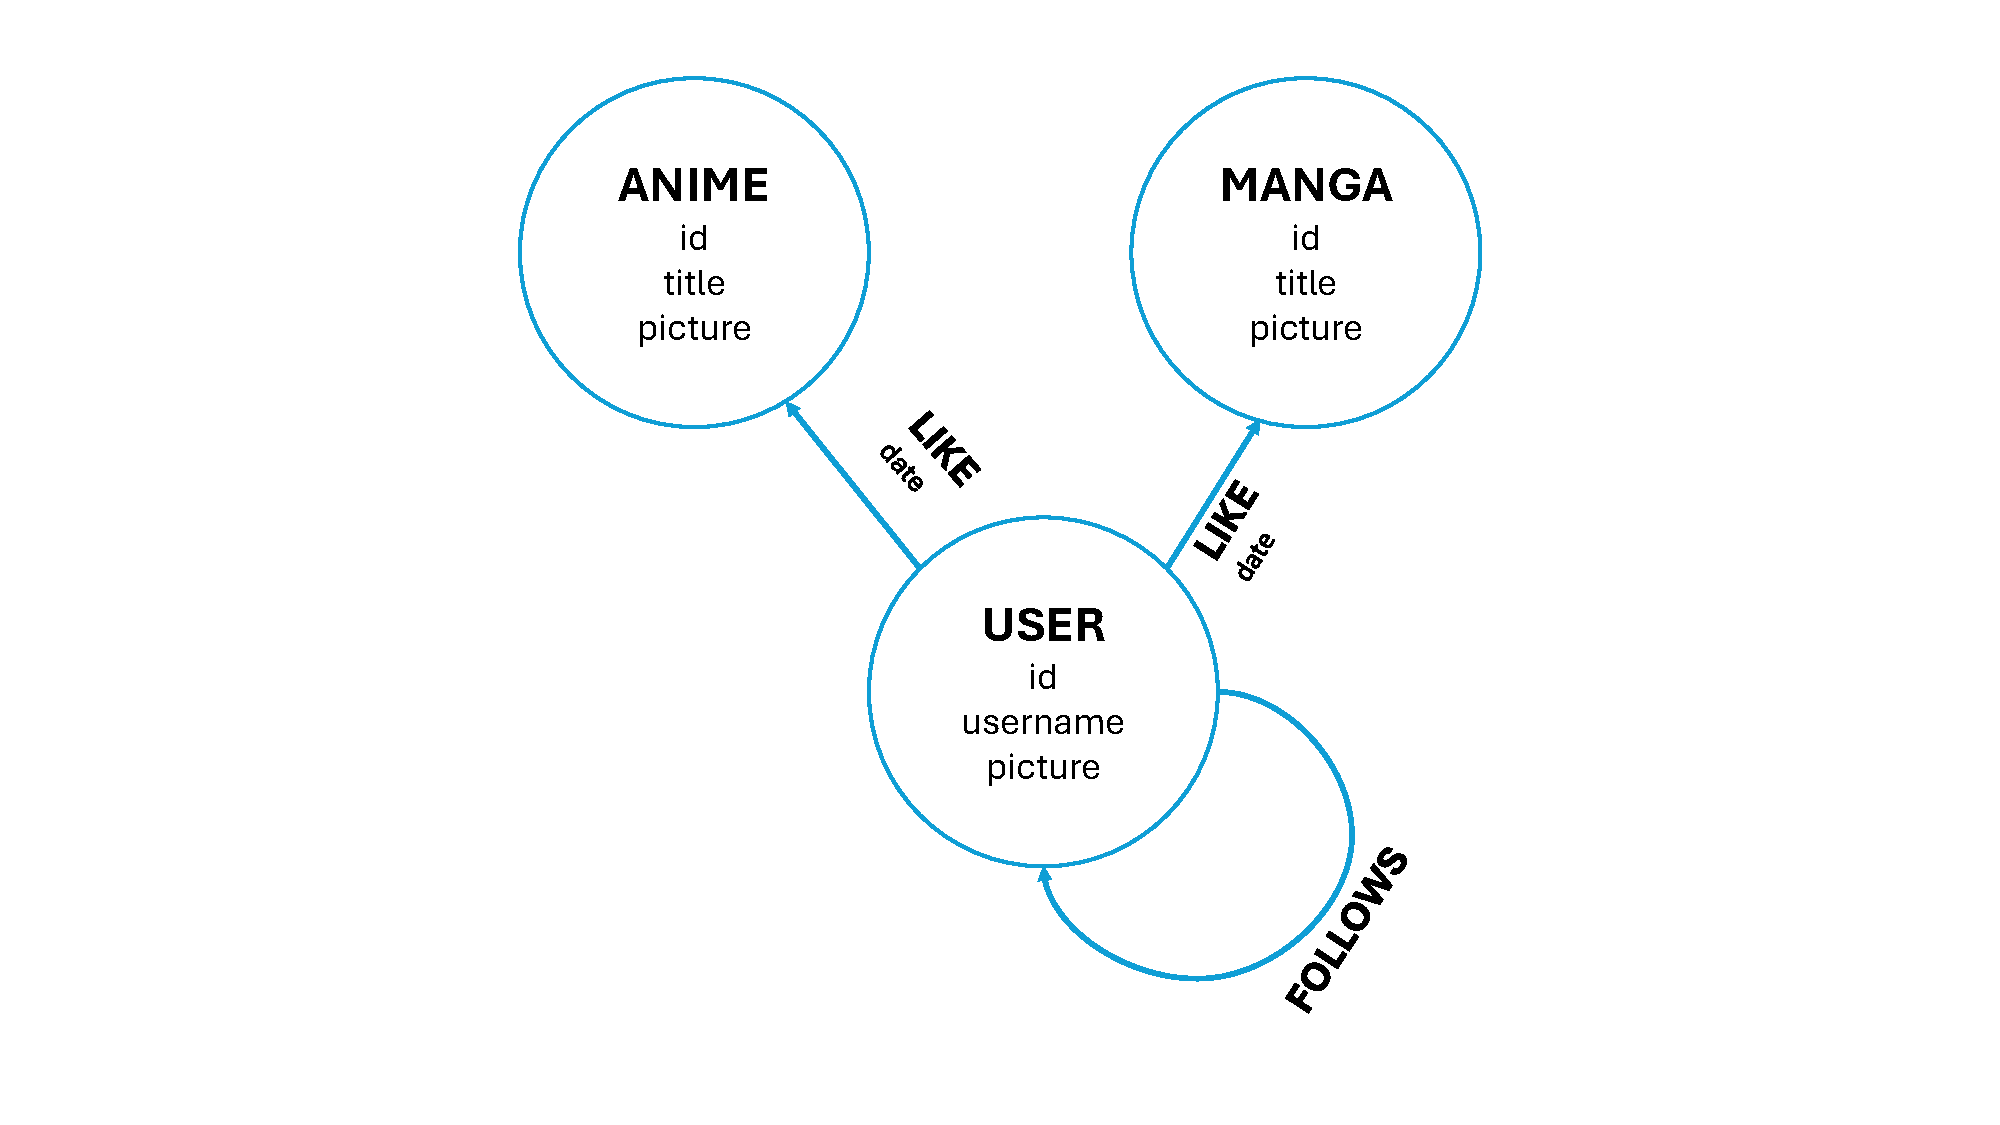
\includegraphics[width=\textwidth]{Media/graph.pdf}
    \caption{GraphDB}
    \label{fig:GraohDB}
\end{figure}

\newpage

\subsection{CRUD operations}
  %% TODO: specify all the crud operations

\begin{itemize}
    \item Create: This operation will allow users to create new nodes and relationships in the database. For example, users can create new relationships between users and media content:
    
    A user can LIKE a media content: 
    \begin{lstlisting}[language=Cypher, caption=Create Like Relationship]
    MATCH (u:User {id: $userId}), (a:Anime {id: $animeId}) 
    WHERE NOT (u)-[:LIKE]->(a) 
    CREATE (u)-[r:LIKE {date: $date} ]->(a)
    RETURN r
    \end{lstlisting}

    A user can FOLLOW another user:
    \begin{lstlisting}[language=Cypher, caption=Create Follow Relationship]
    MATCH (u:User {id: $userId}), (f:User {id: $followedUserId}) 
    WHERE NOT (u)-[:FOLLOWS]->(f) 
    CREATE (u)-[r:FOLLOWS]->(f) 
    RETURN r
    \end{lstlisting}

    \item Read: This operation will allow users to read nodes and relationships from the database. For example, users can read information about anime and manga and relationships between users and media content.
    A user can read the list of liked media contents:
    \begin{lstlisting}[language=Cypher, caption=Read Liked Media Contents]
  
    MATCH (u:User {id: $userId})-[:LIKE]->(a:Anime)
    RETURN a
    \end{lstlisting}

    A user can read the list of followers:
    \begin{lstlisting}[language=Cypher, caption=Read Followers]
    MATCH (u:User {id: $userId})<-[:FOLLOWS]-(f:User)
    RETURN f
    \end{lstlisting}
  
    \item Update: This operation will allow users to update nodes and relationships in the database. For example, users can update their likes for anime and manga and relationships between users.
    
    \item Delete: This operation will allow users to delete nodes and relationships from the database. For example, users can delete their likes for anime and manga and relationships between users.
    
    A user can unlike a media content:
    \begin{lstlisting}[language=Cypher, caption=Delete Like Relationship]
    MATCH (u:User {id: $userId})-[r:LIKE]->(a:Anime {id: $animeId})
    DELETE r
    RETURN r
    \end{lstlisting}
    \newpage
    A user can unfollow another user: 
    \begin{lstlisting}[language=Cypher, caption=Delete Follow Relationship]
    MATCH (:User {id: $followerUserId})-[r:FOLLOWS]->(:User {id: $followingUserId})
    DELETE r 
    RETURN r
    \end{lstlisting}
\end{itemize}

\section {Availability and Partition Tolerance}
MangaVerse, as a social network, gives priority to the AP configuration of the CAP theorem, ensuring Availability and Partition Tolerance. This allows users to access the application and interact with other users and media content, even if the data is not always consistent (Eventual Consistency).

\section{Redundancy}
%what is there to add here?
The performance of the application is critical, so we need to ensure that the system is highly available and fault-tolerant. To achieve this, we gave priority to fast responses, rather than reducing memory consumption.


\textbf{Latest reviews}


In the anime and manga collections, there's a field containing the latest 5 reviews written for that specific media content, in this way it's fast to retrieve. 


\textbf{Average rating}


In the anime and manga collections, there's a field containing the average rating of the media content, this field is updated every time a new review is written.


\textbf{Number of likes}


In the anime and manga collections, there's a field containing the number of likes, this field is updated every time a new like relationship is created or deleted.


\textbf{Followers and Followings}


In the user collection, there are fields containing the number of followers and followings, this field is updated every time a new follow relationship is created or deleted.


\textbf{User field in Reviews}


In the reviews collection, there's a field containing the user data, such as id, username, picture, and also location and birthday, which are used for suggestion porpouses.

\textbf{Media Content field in Reviews}


In the reviews collection, there's a field containg information about the anime or manga the reivew is about. This field has information about the media content id and title.


\textbf{Review Ids}


A list of review ids is stored in the anime, manga and users collections, this is used to quickly retrieve the reviews of a media content and of a user.

\section{Replicas}
A cluster of three nodes is available for this project, allowing deployment of replicas: however, replicas were only implemented in MongoDB, as Neo4j required the Enterprise version for it.
We have 3 replicas for MongoDB and 1 for Neo4J.
In MongoDB we have one primary and two secondary replicas, the primary is used for write operations and the secondaries are used for read operations. This will allow us to distribute the load and improve the performance of the application. In case of failure of the primary node, one of the secondary nodes will be promoted to primary, ensuring high availability of the system.

\newpage
\section{Sharding}
Sharding is a method for distributing data across multiple machines to meet the demands of data growth. As the size of the data increases, a single machine may not be sufficient to store the data nor provide an acceptable read and write throughput. Sharding typically solves the problem with horizontal scaling. However, in our application, sharding is not possible due to the nature of the collections and their interdependencies.

Our database consists of four collections: anime, manga, users, and reviews and each collection stores different types of information.
Sharding these collections would be complex due to their interrelated nature. The data in these collections is highly interconnected; for example, reviews reference both anime/manga and users, and each user can have multiple reviews linked to both anime and manga. Distributing such interdependent data across multiple shards would lead to significant overhead in maintaining relationships between documents, potentially causing performance degradation instead of improvement.

Therefore, while the database design is ready for sharding in theory, the practical constraints of our application's structure and the interconnectedness of our collections make sharding infeasible. Implementing sharding would introduce complexity and overhead that could outweigh the benefits of horizontal scaling in this context.

